% NESSF 2014 proposal

\documentclass[12pt]{article}

%% Use pdfTex to insure the margin sizes in Windows

\usepackage{natbib}
%\usepackage{natbib,natbibspacing}
\setlength{\bibsep}{1pt} % spacing for bibliography items
\citestyle{aa} % apj type
%\citestyle{plain} % number style
\usepackage{multicol} % multicolumns for references

% try smaller section title fonts
\usepackage{sectsty}
\sectionfont{\large}
\subsectionfont{\normalsize}

\pdfpagewidth=8.5in
\pdfpageheight=11in

\setlength\topmargin{-0in}
\setlength\headheight{0in}
\setlength\headsep{0in}
\setlength\textheight{9in}
\setlength\textwidth{6.5in}
\setlength\oddsidemargin{0in}
\setlength\evensidemargin{0in}

\usepackage{mathrsfs}
\usepackage{amsmath,amssymb}
\usepackage{verbatim}
\usepackage{wrapfig}

\usepackage{enumitem}

% journal names
\usepackage{aas_macros}

\newcommand{\beq}{\begin{equation}}
\newcommand{\eeq}{\end{equation}}
\def\etal{~et~al.~}
%\def\mps{m~s$^{-1}$}
\def\mps{m/s}
\def\msini{M\sin{i}}
\def\mjup{M_{\rm Jup}}
\def\msol{M_{\odot}}
\def\mearth{M_{\oplus}}
\def\degree{^{\circ}}
\def\leq{\leqslant}
\def\geq{\geqslant}
\def\kepler{{\it Kepler}}
\def\minerva{MINERVA}
\def\hrs{HET/HRS}
\def\keck{Keck/HIRES}

\usepackage{graphicx}
%\usepackage[pdftex,bookmarks, % add hyperlinks
%colorlinks,
%plainpages=false]{hyperref}

\begin{document}

%\tableofcontents
%\newpage

%%%%%%%%%%%%%%%%%%%%%%%%%%%%%%%%%%%%%%%%%%%%%%%%%%%%%%%%%%%%%%%%%%%%%%%%%%%%%%%%%%%%%%%%%
% title
\title{\vspace{-45pt} \bf \Large Finding the Lowest Mass Exoplanets with
  \\ Improved Radial Velocimetry \vspace{-15pt}}
\author{\normalsize Sharon Xuesong Wang}
\date{}
\maketitle

%%%%%%%%%%%%%%%%%%%%%%%%%%%%%%%%%%%%%%%%%%%%%%%%%%%%%%%%%%%%%%%%%%%%%%%%%%%%%%%%%%%%%%%%%
\vspace{-48pt}
\section{Overview}
\vspace{-5pt}

% An overview of awesomeness of finding low-mass exoplanets.
The great synergy between NASA's \kepler\ mission and the ground-based
radial velocity (RV) surveys has made ground-breaking discoveries of
exoplanets, including many interesting low-mass \citep{marcy2014} and
likely rocky planets \citep{weiss2013} such as Kepler-78b, the first
exoplanet known to have radius and mass very close to Earth's
\citep{howard2013,pepe2013}. In the post-Kepler era, radial
velocimetry will continue to play a key role in validating Kepler
candidates and measuring their masses, as well as discovering
exoplanets independently.

% But... precise RV is yet to be more precise.
However, the current RV precision ($\gtrsim
0.5$--1~\mps)\footnote{The photon-limited precision of the leading RV
  instruments (HARPS and Keck) is $\sim$0.5--1~\mps\ for bright stars,
  while in reality, there is almost always some extra error, i.e.~the
  ``RV jitter", comprised of systematic errors and unaccounted
  stellar-activity signals. For example, the RMS of RV residuals
  against best-fit model for the Kepler-78b system is $\sim 2.5$~\mps,
  with an RV jitter of $\sim 2.1$~\mps, while the photon-limited error
  for the star is $<2$~\mps\ \citep{howard2013,pepe2013}.} is limiting
our ability to detect exoplanets with even lower masses or rocky
planets orbiting farther out, especially in or near the Habitable
Zone. Breaking this limit is critical for enriching the diversity of
the exoplanet ensemble towards lower masses, and it is a necessary
step for finding Earth analogs in the Habitable Zone around Sun-like
stars, which requires an RV precision of $\sim$0.1~\mps.

% What we propose to do
\textbf{We propose to improve the RV precision of several leading RV
  instruments by eliminating $>1$~\mps\ of systematic errors, with the
  aim to find the lowest mass exoplanets.} We will improve the RV
precision of Keck and the 9.2m Hobby-Eberly Telescope (HET), which are
the leading facilities for extensive \kepler\ follow-up observations
as well as independent large and deep RV surveys. Our work will also
improve the RV precision of two instruments on small telescopes:
CHIRON and the upcoming MINiature Exoplanet RV Array
(\minerva). Designed for carrying out dedicated surveys with extremely
high RV precision, CHIRON and \minerva\ will provide valuable high
cadence data on nearby and bright stars, which are the best targets
for planetary atmosphere characterization studies.

\textbf{With improved RV precision, we will revisit and perform
  dynamic analysis on systems with multiple planets, especially the
  ones with small RV amplitudes, such as 55 Cancri, GJ 876, upsilon
  Andromedae, and GJ 581.}


%%%%%%%%%%%%%%%%%%%%%%%%%%%%%%%%%%%%%%%%%%%%%%%%%%%%%%%%%%%%%%%%%%%%%%%%%%%%%%%%%%%%%%%%%
\vspace{-10pt}
\section{Expected Scientific Outcome and Impact}
\vspace{-5pt}
% Keck
\textbf{Science with \keck: } The primary instrument we work with is
the High Resolution Echelle Spectrometer (HIRES) on Keck I (current RV
precision $\sim$1~\mps). Among the 432 RV discovered exoplanets,
\keck\ has contributed the most ($\sim$200). It has also contributed
to a great number of mass measurements of confirmed \kepler\ planets
--- in particular, \textit{most} of the low mass ones
\citep[e.g.,][]{gautier2012,gilliland2013,howard2013,marcy2014}. However,
its current RV precision is limiting its ability to detect even lower
mass planets or planets with the same mass but orbiting farther out
(see, e.g., the marginal or null detections of the confirmed
\kepler\ planets in \citealt{marcy2014}).

% Lots of low mass Kepler planets
Our work will improve the RV precision of \keck, and thus extend the
lower mass limit of the current exoplanet sample. This is especially
promising when considering the large pool of low mass planet
candidates that \kepler\ provides: among the $\sim$1600 KOIs with
transit signals suggesting a planet radius $<$ 2 Earth radii, there
are $\sim$260 whose host stars have \kepler\ magnitude $< 13$ ---
bright enough for Keck to follow up (vs.~fewer than 10 such targets
with \kepler\ mag $< 9$ and thus accessible to HARPS-N; exoplanets.org).

% Multi-planet systems to improve with Keck
Meanwhile, better RV precision will improve the characterization of
multiple-planet systems, especially the ones that host challenging low
RV amplitude planets/candidates and with potentially very active
dynamic interactions. Such systems are valuable samples for studying
the architecture of exoplanet systems and planet formation. We will
reanalyze the RV data and perform dynamic analyses on several of these
systems, including the GJ 876 system, which is the closest
multi-planet systems to the Sun and the only known exoplanet system
with a triple conjunction \citep{marcy2001,rivera2005,rivera2010}; the
$\upsilon$ Andromedae system, the first multi-planet system discovered
around main-sequence star \citep{butler1999,wright2009,curiel2011}; as
well as the GJ 581 system, which hosts the first claimed
terrestrial-mass exoplanet in the Habitable Zone (\citealt{vogt2010},
though it is under debate,
e.g.~\citealt{gregory2011,vogt2012,robertson2013}).

% HET
\textbf{Science with \hrs: } We will also improve the RV precision of
the High Resolution Spectrograph (HRS) on HET (current RV precision
$\sim$3--5~\mps). With multiple ongoing upgrades on \hrs\ (expected to
finish in Summer 2014), its throughput will be improved by a factor of
$\sim$5, also with the promise of higher RV precision of the new
HRS. HET will become the second telescope, besides Keck, capable of
extensive RV follow-up on planet candidates discovered by
\kepler. This will also benefit other planet search programs on
\hrs\ such as surveys on long-period planets and multiple-planet
systems.

% Minerva and CHIRON
\textbf{MINERVA and CHIRON: } The upcoming \minerva\ will consist of
an array of four 0.7m telescopes and a vacuum-sealed, highly-stable
spectrograph (schedule to be online in 2015). It will perform
dedicated RV monitoring on a carefully-selected ensemble of nearby
stars. It is expected to discover $\gtrsim 10$ Earth- to
super-Earth-size planets with orbital period of 1--100 days around
nearby stars, with 3--5 expected to be in the Habitable Zones of their
host stars \citep{bottom2013,hogstrom2013}. Our work will prepare
\minerva\ to meet its targeted long-term RV precision of $\sim
0.8$~\mps.

CHIRON (on the 1.5m SMARTS telescope at CTIO) has demonstrated
short-term RV stability of $\sim0.5$~\mps\ on $\tau$ Ceti
\citep{chiron2013}. The improvement we propose will help CHIRON
achieve long-term RV stability below 1~\mps\ and help validate or
characterize the potential planetary systems around $\tau$ Ceti
\citep{tuomi2013} and $\alpha$ Centauri B
\citep{dumusque2012,hatzes2013}, whose planets (candidates) have RV
amplitudes on the order of $\sim 1$~\mps\ or even smaller.


%%%%%%%%%%%%%%%%%%%%%%%%%%%%%%%%%%%%%%%%%%%%%%%%%%%%%%%%%%%%%%%%%%%%%%%%%%%%%%%%%%%%%%%%%
\vspace{-10pt}
\section{Methodology}
\vspace{-5pt}

% overall
We have identified several underlying causes for RV systematic errors
through our pilot study. Some of these errors are being recognized and
studied in detail \textit{for the very first time}. A few of them
enter the RV error budget at a $\sim 1$~\mps\ or even larger level,
and thus they set the floor for long-term RV precision at 1~\mps\ if
not carefully studied and corrected for. We will determine the first
comprehensive error budget of iodine radial velocimetry.

%---------------------------------------------------------------------------------------
\vspace{-10pt}
\subsection{Removing the Systematics Caused by Telluric
  Lines}\label{sec:tell}
\vspace{-5pt}

% telluric lines act like stellar line impostors but don't shift
In precise iodine radial velocimetry, RVs are measured from the
differential shift of stellar lines between two stellar spectra.
Since all current RV instruments are ground-based, the stellar spectra
inevitably contain telluric absorption lines as from the light's
travel through Earth's atmosphere. These telluric lines impersonate
stellar lines but do not exhibit Doppler shifts caused by the Earth's
barycentric motion ($\sim$a few to tens of k\mps) and the exoplanets. The
resulting ``peak-pulling" effect in the iodine analysis (see,
e.g.~\citealt{wright2013}) then manifests as an annual systematic
signal.

% before we thought it was ok, then we recognized and showed for the
% first time that it's not
For years, such problems caused by telluric lines were thought to have
been suppressed to a negligible level, because there are only few
telluric bands mostly with shallow lines within the working wavelength
region of iodine radial velocimetry (5000\AA--6000\AA). However, as
the RV precision improved over time and has approached
$\sim1$~\mps\ and better, the adverse effects of telluric lines have
emerged and become one of the current bottlenecks of precise radial
velocimetry. \textbf{This is demonstrated \textit{for the first time}
  through our preliminary study, and with some initial effort in
  telluric line masking, we were able to eliminate a visible amount of
  the systematic RV errors}, which is illustrated in
Figure~\ref{fig:tell}.

\begin{figure}[thb]
  \vspace{-3pt}
  \begin{center}
%    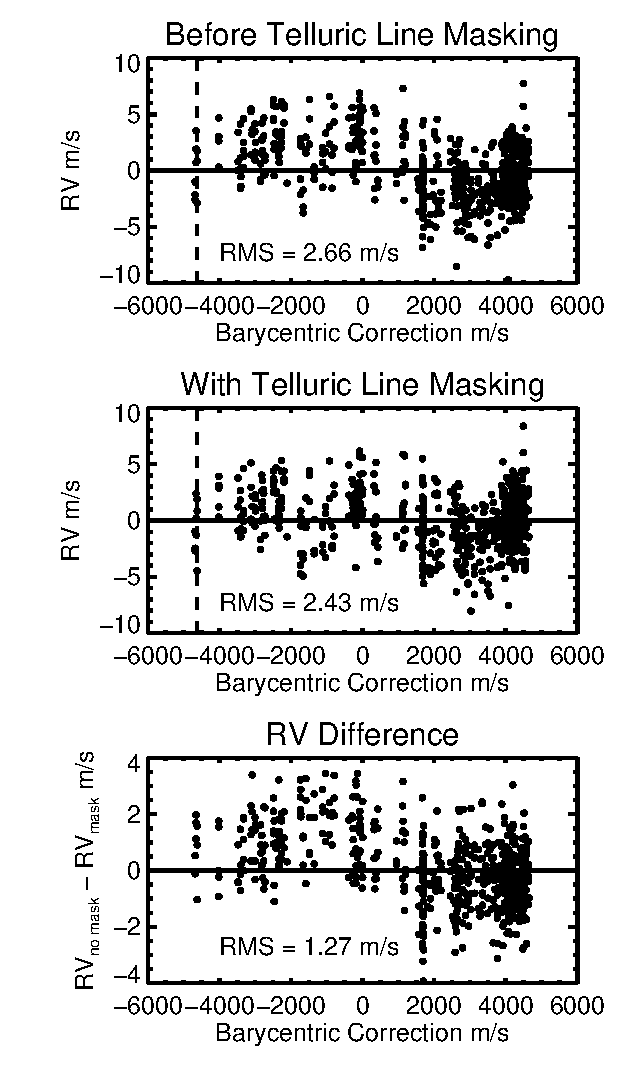
\includegraphics[scale=0.6]{telluric}
    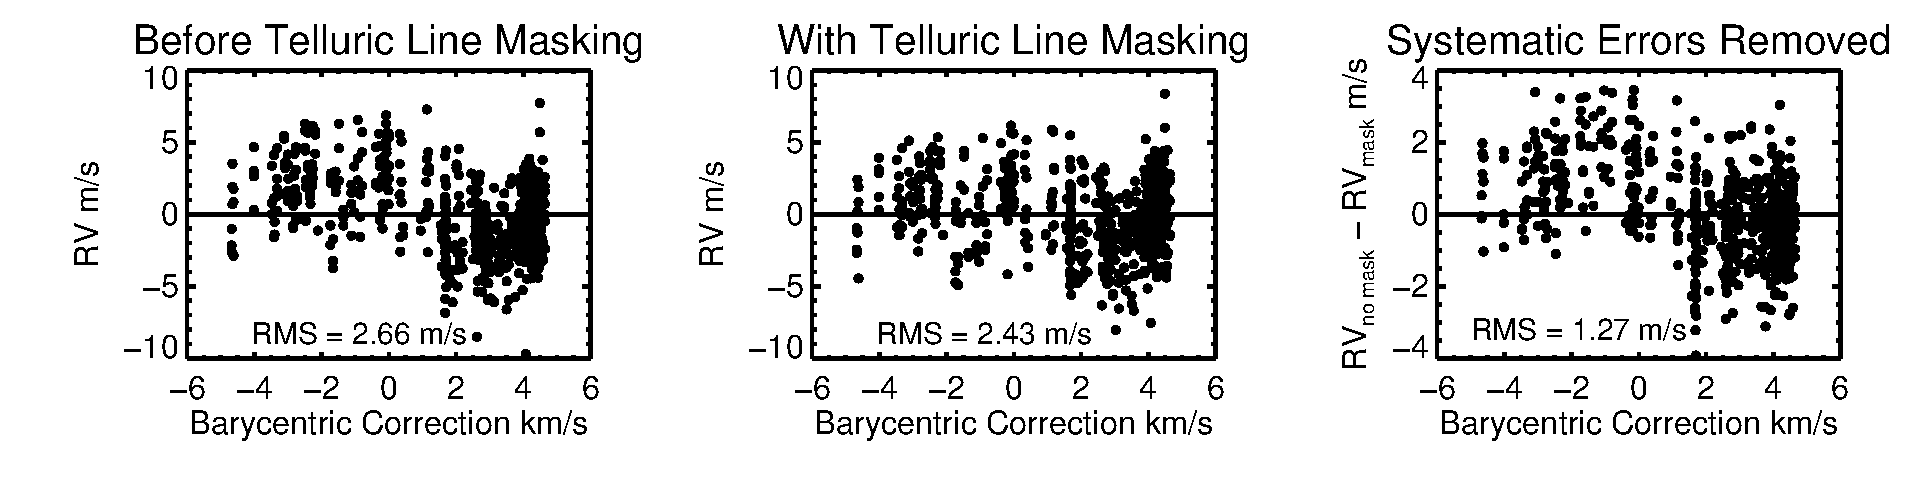
\includegraphics[width=\textwidth]{telluric2}
  \end{center}
  \vspace{-25pt}  
  \caption{Measured precise radial velocities of a standard star
    observed with \keck\ as a function of barycentric correction
    (i.e.~Earth's radial velocity away from the target). Our
    preliminary treatment of telluric lines has removed over
    1~\mps\ systematic noise (panel 3; note the change in scale on
    y-axis).} 
  \vspace{-8pt}  
  \label{fig:tell}
\end{figure}

Figure~\ref{fig:tell} shows that the long-term ($> 5$ years) RV RMS of
an RV standard star observed by \keck, HD 185144 ($\sigma$ Draconis),
is reduced from 2.66~\mps\ to 2.43~\mps\ --- \textbf{an RMS of
  1.08~\mps\ is removed from the RV jitter}
($\sqrt{2.66^2-2.43^2}$). The last panel of Figure~\ref{fig:tell}
illustrates the removed systematic errors, which has a clear annual
signal. The rest of the RV jitter may be due to residual telluric line
effects, intrinsic stellar jitter, other unknown systematic errors, or
even low RV amplitude planets.

% this is only the beginning - lots of improvements can be done!
We will further reduce the systematics caused by telluric lines in
several ways. For example, currently we are masking out the telluric
lines by using a naive simulated telluric spectrum based on the
elevation of Mauna Kea with nominal atmospheric compositions and
conditions. In the future we will employ empirical masks derived from
B star observations. Another example is that the RV extraction code is
not yet optimized to consistently produce a good fit in regions where
some of the pixels are being masked out due to telluric lines,
especially for the cases with large barycentric velocity shifts. A
more carefully-tuned $\chi^2$ minimization algorithm will allow us to
recover reliable RVs from \textit{all} segments of the iodine-laced
stellar spectrum, including those with significant telluric
contamination.

% also HET, MINERVA and CHIRON!
This work will naturally improve the RV precision of \hrs\ and
\minerva, as they share essentially the same RV extraction code
inherited from the \keck\ pipeline. Moreover, the sites of \hrs\ and
\minerva\ are at much lower elevations than Mauna Kea, which means
that the telluric line contamination probably causes more severe
systematic errors. We will also work with the CHIRON team to implement
the treatment for telluric lines to help CHIRON achieve higher
long-term RV precision.


%---------------------------------------------------------------------------------------
\vspace{-10pt}
\subsection{Improving the Wavelength-Dependent Statistical Weighting}\label{sec:vank}
\vspace{-5pt}

\begin{wrapfigure}{r}{0.45\textwidth}
  \vspace{-25pt}
  \begin{center}
    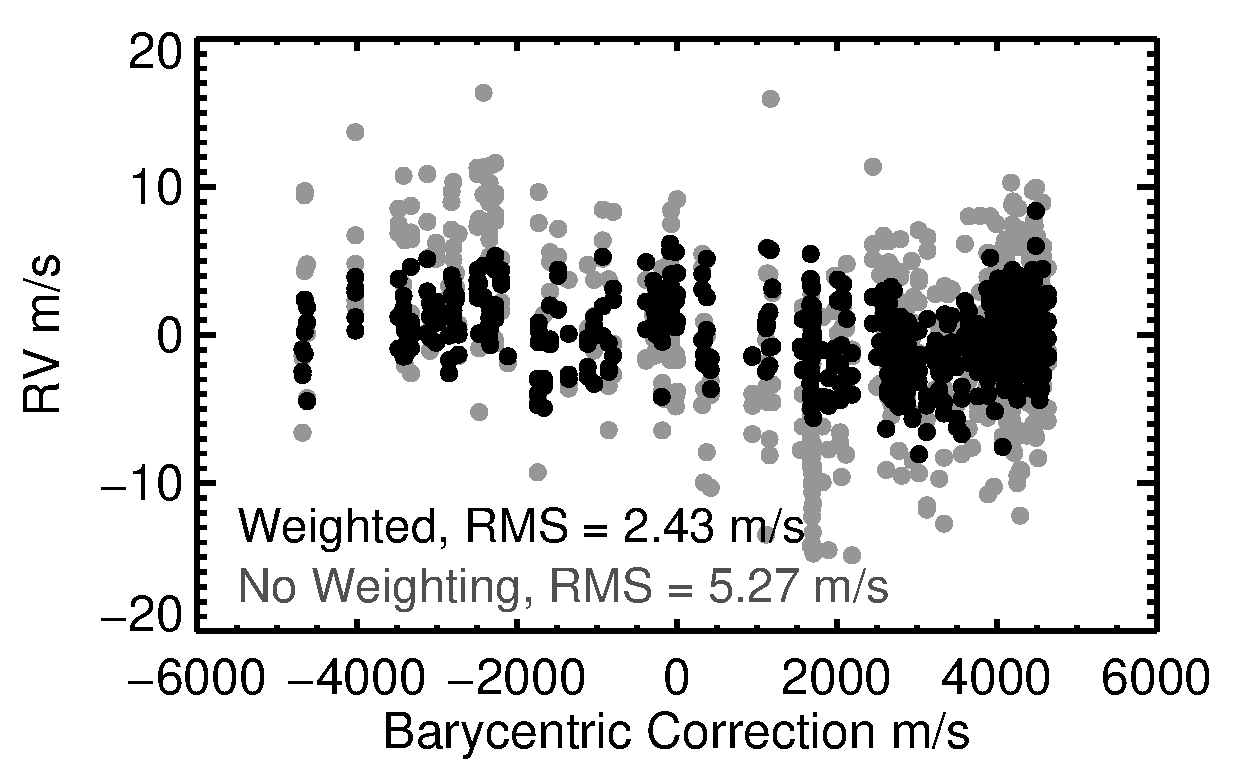
\includegraphics[width=0.42\textwidth]{vank}
  \end{center}
  \vspace{-25pt}  
  \caption{RV RMS of HD 185144 before (gray) and after (black) weighting.} 
  \vspace{-8pt}  
  \label{fig:vank}
\end{wrapfigure}

% what is weighting and its importance
The application of wavelength-dependent statistical weights is the
``secret sauce" of precise iodine radial velocimetry. It evaluates the
RV performance of each wavelength region (an ``RV chunk") across
observations and assigns them statistical weights before computing the
final mean RV. It also adjusts for the wavelength-dependent systematic
offsets and rejects outlier chunks with poor RV RMS
performance. Figure~\ref{fig:vank} illustrates the crucial role of
this weighting scheme in precise radial velocimetry.

% what's 'wrong' with it
Through our preliminary work with telluric lines, we discovered that
the weighting procedure does not give proper treatment to the
telluric-contaminated chunks. It does not incorporate any prior
knowledge on the intrinsic quality of chunks, and consequently, the
telluric-contaminated ones tend to be either brutally rejected or
taken in almost equally as the clean chunks.

% what we plan to do
\textbf{We propose to improve the statistical weighting by
  incorporating prior knowledge on the intrinsic quality of different
  wavelength regions.} Our work will extend beyond implementing proper
treatment for the telluric regions: the current weighting procedure is
purely a post-RV-reduction outlier rejection process, and we will
increase its power by exploiting more prior knowledge on each chunk,
such as the amount of Doppler information content, the signal-to-noise
ratio, and instrumental effects.


%---------------------------------------------------------------------------------------
\vspace{-10pt}
\subsection{Validating the Calibrator: the Iodine Atlas}\label{sec:fts}
\vspace{-5pt}

A ``ground truth" iodine atlas is crucial for the precise iodine radial
velocimetry. It is used for modeling the observed iodine lines in the
stellar$+$iodine RV observation to anchor the absolute wavelengths and
the spectrograph response function. Such a ``ground truth" atlas is
normally obtained through a Fourier Transform Spectrometer
(FTS). However, our recent work has revealed potential problems with
the quality of FTS iodine atlases.

We took a new FTS atlas of the \hrs\ iodine cell at NIST and compared
it with the old one (taken at KPNO in 1993), which showed that they
differ significantly in terms of wavelength scales and line
shapes. The RV jitter of the RV standard star HD 185144 (observed with
\hrs) is $\sim5$~\mps\ when we use the new FTS atlas
vs.~$\sim4$~\mps\ with the old one. This calls into questions of how
``true" any existing FTS iodine atlas really is, and demands for an
independent method to validate them. \textbf{We propose to validate
  the quality of the FTS iodine atlases for the new \hrs\ and
  \minerva, and also for CHIRON and other RV instruments if
  necessary.}

We have found a method to independently validate the quality of FTS
iodine atlas, which is to take a high-resolution echelle spectrum of
the iodine cell in the ``real wavelength space" (as opposed to in
Fourier space with FTS). We used the TS12 arm of the Tull Spectrograph
at the McDonald Observatory 2.7m telescope, which has the matching
spectral resolution to an FTS ($R \sim 500,000$). For our pilot study,
we used the iodine cell at the McDonald 2.1m telescope, whoese FTS
atlas was also taken at KPNO in 1993 and thus can represent the
quality of the KPNO FTS atlases.

\begin{wrapfigure}{r}{0.5\textwidth}
  \vspace{-35pt}
  \begin{center}
    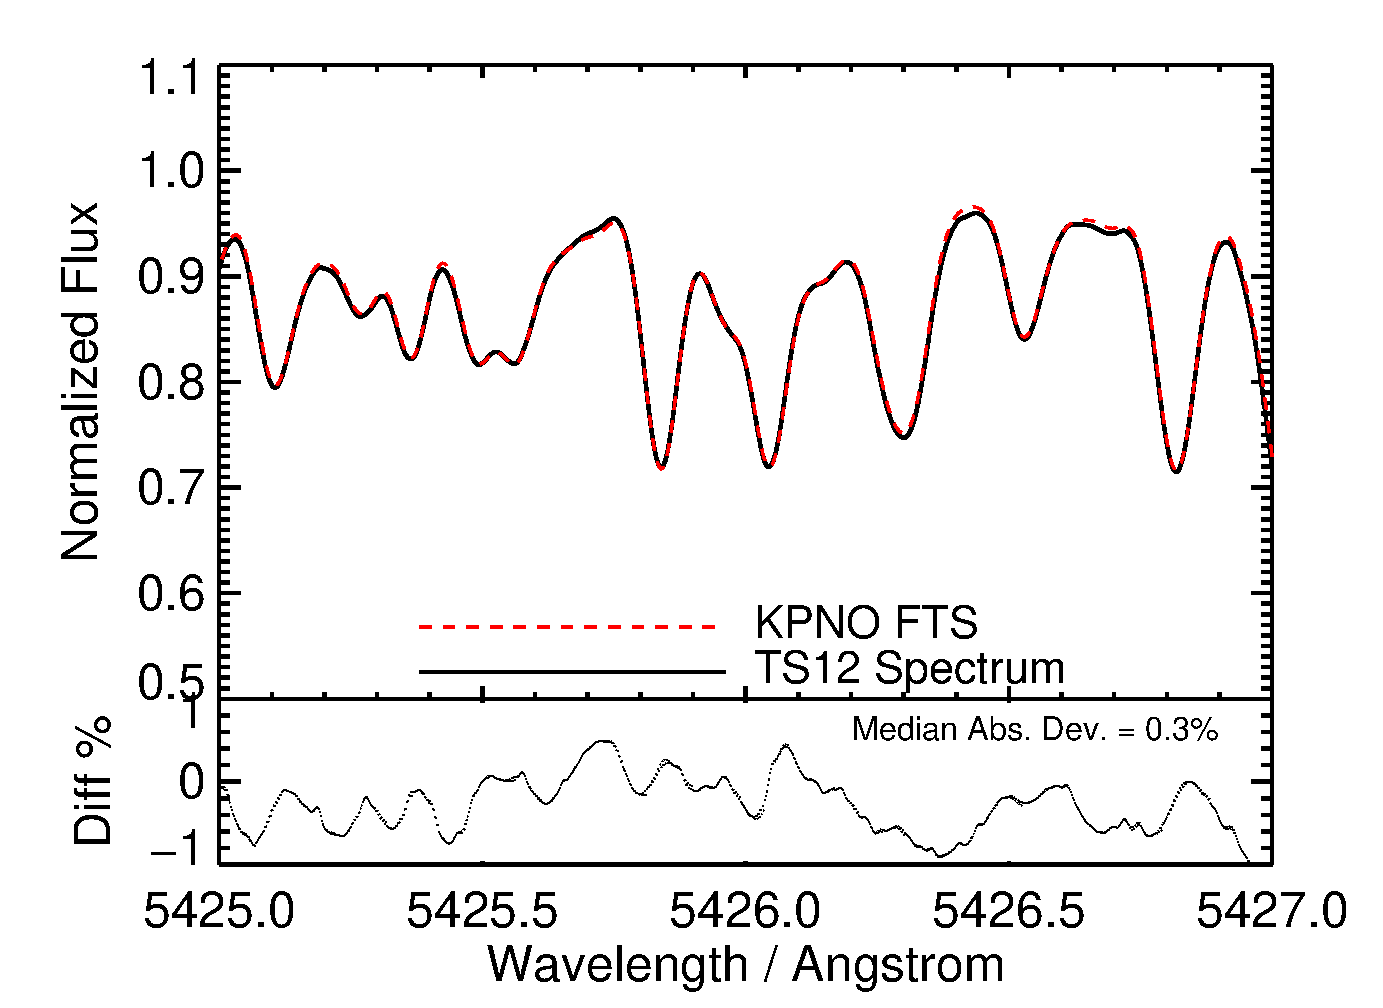
\includegraphics[width=0.47\textwidth]{fts}
  \end{center}
  \vspace{-25pt}  
  \caption{FTS iodine atlas compared with echelle spectrum, both
    at $R=60,000$.}  
  \vspace{-8pt}  
  \label{fig:fts}
\end{wrapfigure}

Figure~\ref{fig:fts} illustrates the comparison between the FTS iodine
atlas and the echelle spectrum (zoomed into a 2\AA\ chunk). It shows
that, when convolved down to resolution $R=60,000$ (typical resolution
of an star$+$iodine RV observation), the difference between the KPNO
scan and the echelle spectrum is consistent with photon-limited
errors and potential errors in flat fielding and scattered light
removal.

This demonstrates that we have found an independent and reliable
method to validate any FTS iodine atlas. Current and upcoming RV
instruments such as the new \hrs, \minerva, and CHIRON will need
validation for their FTS iodine atlases to eliminate one risk factor
that could potentially compromise the RV precision, which is our
proposed work here.

%---------------------------------------------------------------------------------------
\vspace{-10pt}
\subsection{Improving Data Reduction and Instrument Modeling}\label{sec:ip}
\vspace{-5pt}

We propose to improve the data reduction pipeline of \hrs\ in
preparation for its upgrade (schedule to finish in Summer 2014) and
also for the upcoming project \minerva. The new \hrs\ will have a new spectral
format that is similar to CHIRON and \minerva. This new format will
have five parallel images for each echelle order due to the
implementation of an image slicer, and this poses a challenge to data
reduction, especially for flat fielding. With our experience of
setting up data reduction pipeline for the current
\hrs\ \citep{wang2012} and our close collaboration with the CHIRON
group, we will produce a pipeline for the new \hrs\ and
\minerva\ to ensure the delivery of high RV precision.

Another factor that is limiting the current precision of \hrs\ is the
modeling of the spectrograph response function (SRF). This is probably
not a dominant issue for \keck, since the SRF of HIRES has been
studied in detail and modeled successfully. However, for the fiber-fed
\hrs\ and \minerva, the SRF will be significantly different and
require more careful study on fiber spectroscopy. We have acquired
on-sky and engineering test data with \hrs\ designed to address this
issue, as well as the issue of modal noise, which is also unique to
fiber-fed spectrographs.

 
%%%%%%%%%%%%%%%%%%%%%%%%%%%%%%%%%%%%%%%%%%%%%%%%%%%%%%%%%%%%%%%%%%%%%%%%%%%%%%%%%%%%%%%%%
\vspace{-10pt}
\section{Relevance to NASA's Objectives and Missions}
\vspace{-5pt}

Broadly, our investigation addresses one of the science
objectives of NASA SMD, ``Discover the origin, structure, evolution
and destiny of the universe and search for Earth-like planets".

More specifically, this proposal is directly and closely relevant to
the Astrophysics Research Program, theme (iii) Exoplanet Exploration,
in the solicitation: \textbf{(1)``to search for planets and planetary
  systems about nearby stars in our Galaxy":} This is the direct
science goal of our work. \textbf{(2) ``to determine the properties of
  those stars that harbor planetary systems":} We will acquire high
resolution spectra on planet host stars with \keck\ and \hrs\ for,
e.g. the \kepler\ stars, as required by the RV technique. Improved RV
precision will also help better understanding stellar activities and
stellar RV jitter. \textbf{(3)``to determine the percentage of planets
  that are in or near the Habitable Zone of a wide variety of stars
  and to measure their orbits":} Improved RV precision of \keck\ and
\hrs\ will enable more detections of potentially rocky exoplanets in
the Habitable Zone of their host stars, which is also the immediate
goal of project \minerva.

Our work will support current and future NASA missions: We will
enhance the scientific outcome of the \textbf{\textit{Kepler} mission}
through follow-up programs such as candidate validation, planetary
mass measurements, and TTV target follow-up. In the future, \keck,
\hrs, and \minerva\ can all contribute significantly to the follow-up
programs of \textbf{TESS}. Improved radial velocimetry will find more
super Earths and Earth analogs, which are the primary targets for
\textbf{JWST} for planetary atmosphere characterization.


%%%%%%%%%%%%%%%%%%%%%%%%%%%%%%%%%%%%%%%%%%%%%%%%%%%%%%%%%%%%%%%%%%%%%%%%%%%%%%%%%%%%%%%%%
%\newpage
%\addcontentsline{toc}{section}{References}
\vspace{-3pt}
\bibliographystyle{apj}	% (uses file "xxx.bst")
%\begin{multicols}{2}
{\small % smaller fonts for references
%{\footnotesize
\bibliography{references} }
%\end{multicols}

%%%%%%%%%%%%%%%%%%%%%%%%%%%%%%%%%%%%%%%%%%%%%%%%%%%%%%%%%%%%%%%%%%%%%%%%%%%%%%%%%%%%%%%%%
% RECYCLE BIN
\begin{comment}
% overview
\textbf{We propose to improve the RV precision of several leading RV
  instruments through correction of systematic errors, with the aim to
  find the lowest mass exoplanets.} Improved radial velocimetry will
also enable better characterization of the currently known low RV
amplitude planetary systems. Moreover, eliminating instrumental
systematic errors will help in isolating the RV signals induced by
stellar activities and promote a better understanding of the stellar
RV jitter, which is also crucial for finding lower mass exoplanets.
  
The excellent synergy between NASA's \kepler\ mission and the
ground-based radial velocity (RV) surveys has made numerous
ground-breaking discoveries of exoplanets, including many interesting
low-mass and rocky planets
\citep[e.g.,][]{howard2013,pepe2013,marcy2014}. This has brought the
field of exoplanets into an exciting era with an inceasing sample of
small and potentially rocky planets \citep{weiss2013} with the great
promise towards the discovery of Earth analogs in the near future.

In the post-\kepler\ era, radial velocimetry will undoubtedly continue
to play a key role in validating \kepler\ candidates and measuring
their masses, as well as discovering exoplanets
independently. However, the current precision of radial velocimetry
(0.5--1~\mps) acts as one of the major limiting factors in detecting
exoplanets with even lower masses or rocky planets further out in the
orbit, especially in or near the Habitable Zone. Breaking this limit
is critical for pushing the lower mass boundary of the exoplanet
ensemble. It is also an absolutely necessary step towards finding
Earth-mass ($\mearth$) exoplanets in the Habitable Zone around
Sun-like stars, which requires an RV precision of $\sim$0.1 \mps.
  
The field of exoplanet is progressing in a fast pace towards the
discovery of Earth-like planets around other stars. During the past
decades, we have moved on from the age of booming discoveries of
Jupiter-mass exoplanets via radial velocimetry (add ref) to the
\kepler\ era where there are thousands of Earth- and super-Earth-size
exoplanet candidates (add ref). Moreover, great promises lie ahead with
future ground-based instruments (e.g., ESPRESSO; add ref) or space
missions (e.g., TESS; add ref).

% science
Our work also has great synergy with two
very high RV precision instruments on smaller telescopes: the upcoming
\minerva\ and CHIRON on the 1.5m SMARTS telescope at CTIO. 

is limiting its ability to detect lower mass
planets or planets with the same mass but further out in orbit
\citep[e.g.,][]{marcy2014}.

% example of listed item
\begin{itemize}[leftmargin=2.2em]
    \vspace{-3pt}
\item Improve the RV precision of Keck through eliminating known
  systematics and improved statistics.
    \vspace{-3pt}
\end{itemize}

% methodology overview
Our approach for improving the RV precision is to eliminate the RV
systematic errors, one of the two major contributors to the 'RV
jitter' (the other being stellar jitter).

We propose to work on: removal of RV systematic errors / annual jitter
cause by the Earth's atmospheric absorption (telluric lines;
Section~\ref{sec:tell}); improvements in wavelength-dependent
statistical weighting in spectrum for RV extraction
(Section~\ref{sec:vanking}); validation of the RV calibrator, the
iodine atlas, using high-resolution echelle spectrograph
(Section~\ref{sec:fts}); and improvements in data reduction and
instrumental effect modeling for fiber-fed RV instruments
(Section~\ref{sec:ip}). 

% FTS
Doppler reductions on the RV standard star HD 185144 yield a
RV jitter of $\sim5$~\mps\ when using the new FTS atlas and
$\sim4$~\mps\ with the old one.

We took a 30\AA\ chunk of echelle absorption spectrum of
the iodine cell at the McDonald 2.1m telescope and compared it with
its FTS iodine atlas (also taken at KPNO in 1993 and thus can
represent the quality of the KPNO FTS spectra).

One key element in precise RV work with iodine is the ``ground truth"
of the absorption spectrum of the iodine cell, which is normally a
wavelength-calibrated, very high-resolution iodine atlas taken by a
Fourier Transform Spectrometer (FTS). Treated as the ``true and perfect
iodine spectrum", the FTS iodine atlas is used for modeling the iodine
lines in the observed stellar$+$iodine spectrum to anchor the absolute
wavelength solution and the spectrograph response function. Therefore,
an accurate and precise iodine atlas is crucial for achieving high RV
precision.

When extracting RVs from the stellar spectrum obtained through an
iodine cell, one relies on the modeling of the iodine lines using the
``true lines" in the iodine atlas to anchor the absolute wavelength
solution and the spectrograph response function (the ``spectral PSF").

Modeling the observed iodine lines using this ``ground truth" iodine
atlas anchors the absolute wavelength solution and the spectrograph
response function (the `spectral PSF' or instrumental profile, `IP')
when extracting RVs from the stellar spectrum.

Modeling the observed Iodine lines with the FTS scan spectrum anchors
the absolute wavelength solution and spectrograph response function
when extracting RVs from the stellar spectrum.

% data reduction and IP
This part is for improving RV of fiber-fed spectrographs: \hrs,
\minerva, and CHIRON.

The new \hrs\ is going to have a different spectral format, which is
very similar to what \minerva\ will have. We need to modify the data
reduction and doppler code for \hrs\ to adapt to it to ensure it
reaches the optimized precision. This will naturally also be
preparation work for \minerva. Addressing the challenge of flat
fielding for such spectral format will also help improve CHIRON.

Another crucial work is to model the instrumental profile of fiber-fed
spectrograph really well and to understand the problems that are
unique for fibers. IP is very important and \hrs\ is not doing very
well. We have acquired lots of engineering data on
\hrs\ to specially designed for modeling IPs and understanding modal
noise of fibers. Combined with years of engineering data and
experience with CHIRON, improvement on IP modeling is ahead. This is
also a natural preparation work for \minerva.


% an old section
\section{Relation to PI's Other NASA Grants}
The PI of this proposal, Dr.~Jason Wright, has received NASA Keck
time to search for long-period planet and multiple planet systems.
The PI has also received NASA Keck time to follow up a
\kepler\ planetary system with a strong TTV signal (Co-I Eric
Ford). Both of these programs will of no doubt benefit from the
improved Keck RV precision, and the upgraded \hrs\ is expected to
follow up some if not all of the long-period planet systems and
\kepler\ TTV systems in the future.

% relevance to NASA
\begin{itemize}[leftmargin=1.5em]
  \vspace{-8pt}
\item ``to search for planets and planetary systems about
  nearby stars in our Galaxy": This is the direct science goal of our
  work. 
  \vspace{-5pt}
\item ``to determine the properties of those stars that harbor
  planetary systems": We will acquire high resolution spectra on
  planet host stars with \keck\ and \hrs\ for, e.g. the
  \kepler\ stars, as required by the RV technique. Improved RV
  precision will also help better understanding stellar activities and
  stellar RV jitter.
  \vspace{-5pt}
\item ``to determine the percentage of planets that are in or near the
  Habitable Zone of a wide variety of stars and to measure their
  orbits": Improved RV precision of \keck\ and \hrs\ will enable more
  detections of potentially rocky exoplanets in the Habitable Zone of
  their host stars, which is also the immediate goal of project \minerva.
  \vspace{-8pt}
\end{itemize}

Our work will also support current and future NASA missions and
enhance their scientific outcome: (1) the Kepler mission: Our work
directly supports the Kepler mission through candidate
validation/confirmation, planetary mass measurements, TTV target
follow-up, and outer planet discovery using Keck/HIRES and
HET/HRS. (2) TESS: Keck/HIRES, HET/HRS, and MINERVA can all contribute
significantly to the follow-up programs of TESS. (3) JWST: Finding
more lower mass exoplanets means more super Earths and Earth analogs,
which are the primary targets for JWST for planetary atmosphere
characterization. 

\end{comment}
%%%%%%%%%%%%%%%%%%%%%%%%%%%%%%%%%%%%%%%%%%%%%%%%%%%%%%%%%%%%%%%%%%%%%%%%%%%%%%%%%%%%%%%%%

\end{document}
